\documentclass[11pt,a4paper,titlepage]{jsarticle}
%
\usepackage{amsmath,amssymb}
\usepackage{bm}
\usepackage{ascmac}
\usepackage{empheq}
\usepackage[dvipdfmx]{graphicx}
\usepackage[dvipdfmx]{color}
\usepackage{float}
\usepackage{siunitx}
\usepackage{enumerate}
\usepackage{booktabs}
\usepackage{subcaption}
\usepackage{autobreak}
\usepackage{longtable}
\usepackage{listings}
%
\SetSymbolFont{letters}{normal}{OT1}{cmr}{m}{n}
\SetMathAlphabet{\mathnormal}{normal}{OT1}{cmr}{m}{n}
%
\setlength{\textwidth}{\fullwidth}
\setlength{\textheight}{40\baselineskip}
\addtolength{\textheight}{\topskip}
\setlength{\voffset}{-0.2in}
\setlength{\topmargin}{0pt}
\setlength{\headheight}{0pt}
\setlength{\headsep}{0pt}
%
\graphicspath{{./figure/}}
%
\everymath{\displaystyle}
%
\makeatletter
\def\@maketitle{
  \begin{flushright}
    {\large \@date}
  \end{flushright}
  \par\vskip 1.5em
  \begin{center}
    {\LARGE \@title \par}
  \end{center}
  \par
  \begin{flushright}
    {\large \@author}
  \end{flushright}
  \par\vskip 1.5em
}
\makeatother
%
\makeatletter
\newcommand{\figcaption}[1]{\def\@captype{figure}\caption{#1}}
\newcommand{\tblcaption}[1]{\def\@captype{table}\caption{#1}}
\makeatother
%
\newcommand{\divergence}{\mathrm{div}\,}  %ダイバージェンス
\newcommand{\grad}{\mathrm{grad}\,}  %グラディエント
\newcommand{\rot}{\mathrm{rot}\,}  %ローテーション
\newcommand{\const}{\mathrm{const.}\,} %一定
%
\newcommand{\us}[2]{\underset{#1}{\vphantom{|_|}#2}}
\newcommand{\ub}[1]{\underbrace{#1}}
\newcommand{\ur}[1]{\underbracket{#1}}
%
\title{}
\author{}
\date{\today}
%
\begin{document}

\section{品詞}

\subsection{品詞の分類}

\subsubsection{名詞(Noun)}
名詞はモノやコトを表す品詞であり、文構造の骨格にかかわってくる品詞である。
文構造の中ではS(主語)、O(目的語)を主に担い、場合によってはC(補語)を担うこともある。
また、複数の単語が集まって名詞句や名詞節を形成すると、その塊で名詞としての役割を担うことがある。\\
e.g., Apple, School, Pen

\subsubsection{動詞(Verb)}
動作や状態などを表す品詞であり、文構造の骨格にかかわってくる品詞である。
文構造の中ではV(述語)を担う。\\
e.g., take, have, live

\subsubsection{助動詞(Auxiliary verb)}
文字通り動詞の意味を補助する役割の品詞である。
動詞とセットで意味を成す。\\
e.g., can, will, must

\subsubsection{形容詞(Adjective)}
名詞(名詞句、名詞節)を修飾する品詞である。
必ず紐づいている名詞がある。
通常の限定用法では文構造の骨格にかかわってこないが、直接S(主語)を叙述するような叙述用法ではC(補語)を担う。\\
e.g., beautiful, cool, high

\subsubsection{副詞(Adverb)}
名詞以外(主に動詞や文全体)を修飾する品詞である。
文構造の骨格にかかわってくることはない。
ある意味、ほかの分類に当てはまらないものが副詞と分類されていると言ってもよい。\\
e.g., always, carefully, just

\subsubsection{接続詞(Conjunction)}
文と文をつないだり、節を導いたりする品詞である。\\
e.g., and, but, if

\subsubsection{前置詞(Preposition)}
文字通り名詞の前に置いて関係を示す品詞であるが、形容詞や副詞の前に置かれるケースもある。\\
e.g., in, on, of

\subsubsection{冠詞(Article)}
名詞の前に置いて、その名刺が特定のものかそうでないかを示す品詞である。\\
e.g., a, an, the

\subsubsection{間投詞(Interjection)}
「わぁ」のように呼びかけを表したりする。\\
e.g., wow, oh, ah

\subsection{品詞決定の重要性}
以下の表を見てみよう。

\begin{table}[h]
  \centering
  \begin{tabular}{ccl}
    \hline
    品詞 & 意味 & \multicolumn{1}{c}{例文} \\
    \hline \hline
    名詞 & 背中、背後 & 
    \begin{tabular}{l}
      There is a bug on my back.\\
      背中に虫がついている。
    \end{tabular} \\
    動詞 & 後援する & 
    \begin{tabular}{l}
      I back this politician.\\
      私はこの政治家を後援している。
    \end{tabular} \\
    形容詞 & 後ろの & 
    \begin{tabular}{l}
      I entered by the back door.\\
      私は裏口から中へ入った。
    \end{tabular} \\
    副詞 & 後ろに & 
    \begin{tabular}{l}
      I came back.\\
      私は戻ってきた。
    \end{tabular} \\
    \hline
  \end{tabular}
\end{table}

例ではbackを挙げたが、名詞・動詞・形容詞・副詞など、使い方が複数ある英単語は枚挙にいとまがない。
例文のように単純明快な文章であればよいが、複雑な文章では、語順、近くの単語の形、文脈上のつながりなどを手掛かりにして、各単語の品詞を決定させなければならない。
品詞の決定(特に動詞)を誤ると、文構造の把握は当然であるが、文の概要の把握にも失敗してしまう。
入試問題で見かける難しい文章というのは、品詞決定しずらい単語を使ったり、入れ子構造を使ったり、転置や省略を多用したりして、巧みに難解な文章を作り上げている。
このような文構造のトリックを看破できるようになれば、英語はもはや敵ではない。


\section{要素と文型}

\subsection{要素}

\subsubsection{主語S(Subject)}
主語の要素を担うのは名詞(名詞句・名詞節)のみである。
どの文型にも必須の要素である。

\subsubsection{述語V(Verb)}
述語の要素を担うのは動詞(動詞句)のみである。
どの文型にも必須の要素である。

\subsubsection{目的語O(Object)}
目的語の要素を担うのは名詞(名詞句・名詞節)のみである。
SVO、SVOO、SVOCに必要な要素である。

\subsubsection{補語(Complement)}
補語の要素を担うのは名詞(名詞句・名詞節)と形容詞(形容詞句・形容詞節)のみである。
SVC、SVOCに必要な要素である。

\subsubsection{修飾語(Modifier)}
修飾語とは、上記の4要素以外のものである。
修飾語の要素を担うのは主に副詞(副詞句・副詞節)である。
文構造にはかかわらない要素なので、文の中にいくつあってもよいし、逆になくてもよい。
よって、5文型のどの構成要素でもない。

\begin{table}[h]
  \centering
  \begin{tabular}{ll}
    \hline
    \multicolumn{1}{c}{要素} & \multicolumn{1}{c}{品詞}\\
    \hline \hline
    主語S & 名詞\\
    述語V & 動詞\\
    目的語O & 名詞\\
    補語C & 名詞・形容詞\\
    修飾語M & 副詞\\
    \hline
  \end{tabular}
\end{table}

\subsection{文型}

\subsubsection{第1文型: SV}
主語Sと述語Vで構成される文。
例えば、純粋にSとVだけで構成されている文章としては、以下のようなものがある。

\begin{equation}
  \ub{\us{代名詞}{I}}_S ~ \ub{\us{動詞}{walk}}_V \text{.}
\end{equation}

他にも、副詞が修飾語Mとして付くようなケースもあるが、修飾語Mは文構造にかかわらないため、同じくSVの構造になる。

\begin{equation}
  \ub{\us{代名詞}{I}}_S ~ \ub{\us{動詞}{walk}}_V ~ \ub{\us{副詞}{slowly}}_M \text{.}
\end{equation}

前置詞に導かれている名詞がある場合は要注意である。
前置詞に導かれている名詞は副詞句を形成するので、修飾語となる。
つまり、文構造の骨格からは省かれる。

\begin{equation}
  \ub{\us{代名詞}{I}}_S ~ \ub{\us{動詞}{walk}}_V ~ \ub{\ur{\us{前置詞}{to} ~ \us{名詞}{school}}_{副詞句}}_M \text{.}
\end{equation}

\subsubsection{第2文型: SVC}
主語Sと述語Vと補語Cで構成される文。
「主語S=補語C」の関係が成り立っている。
補語Cは名詞の場合と形容詞の場合がある。

\begin{equation}
  \ub{\us{代名詞}{This} ~ \us{名詞}{flower}}_S ~ \ub{\us{動詞}{is}}_V ~ \ub{\us{前置詞}{a} ~ \us{名詞}{rose}}_C \text{.}
\end{equation}

\begin{equation}
  \ub{\us{代名詞}{This} ~ \us{名詞}{flower}}_S ~ \ub{\us{動詞}{is}}_V ~ \ub{\us{形容詞}{red}}_C \text{.}
\end{equation}

確かに、$This ~ flower = a ~ rose$と$This ~ flower = red$の関係が成り立っていることがわかる。
SVのときと同様に、修飾語Mがつくケースがある。
繰り返しになるが、修飾語Mは文構造にかかわらないため、同じくSVCの構造になる。

\begin{equation}
  \ub{\us{代名詞}{This} ~ \us{名詞}{flower}}_S ~ \ub{\us{動詞}{is}}_V ~ \ub{\us{副詞}{probably}}_M ~ \ub{\us{前置詞}{a} ~ \us{名詞}{rose}}_C \text{.}
\end{equation}

\subsubsection{第3文型: SVO}
主語Sと述語Vと目的語Oで構成される文。
「主語Sが目的語Oを動詞Vする」の関係が成り立っている。
基本的には動詞Vの直後に目的語Oが来るので、動詞の直後に名詞の役割をするものが続いているとき、必ずそれは目的語Oである。
一般的に、日本語で「○○を」となるときは目的語をとってSVOの構文になると言われている。
おおよそは当てはまっているが、例外は多々あるのでこの覚え方は要注意。

\begin{equation}
  \ub{\us{代名詞}{I}}_S ~ \ub{\us{動詞}{drink}}_V ~ \ub{\us{形容詞}{cold} ~ \us{名詞}{juice}}_O \text{.}
\end{equation}

\subsubsection{第4文型: SVOO}
主語Sと述語Vと目的語$O_1$と$O_2$で構成される文。
「主語Sが目的語$O_1$に目的語$O_2$を動詞Vする」の関係が成り立っている。
基本的には動詞Vの直後に目的語$O_1$が来て、その直後に目的語$O_2$が来る。

\begin{equation}
  \ub{\us{代名詞}{I}}_S ~ \ub{\us{動詞}{give}}_V ~ \ub{\us{代名詞}{you}}_{O_1} ~ \ub{\us{冠詞}{a} ~ \us{名詞}{gift}}_{O_2} \text{.}
\end{equation}

SVOOの構文はSVOの形に書き換えることができる。

\begin{equation}
  \ub{\us{代名詞}{I}}_S ~ \ub{\us{動詞}{give}}_V ~ \ub{\us{冠詞}{a} ~ \us{名詞}{gift}}_O ~ \ub{\ur{\us{前置詞}{to} ~ \us{代名詞}{you}}_{副詞句}}_{M} \text{.}
\end{equation}

意味は同じく「私はあなたにプレゼントをあげる」というものだ。
文法上は、$O_1$の頭に前置詞$to$が付いて修飾語Mになり、$O_2$が目的語Oとなっている。
$O_1$の頭に付くのは主に$to$だが、$for$などのほかの前置詞が付く場合もある。
細かい部分は後に取り上げる。

\subsubsection{第5文型: SVOC}
主語Sと述語Vと目的語Oと補語Cで構成される文。
SVCのときと近いが、今度は「目的語O=補語C」の関係が成り立っている。
意味上は「主語Sが目的語Oを補語Cに動詞Vする」の関係が成り立っている。
動詞の直後に名詞の役割をするものが2連続で来ているときは、SVOOかSVOCの構文を疑おう。
SVCのときと同様に、補語Cは名詞の場合と形容詞の場合がある。

\begin{equation}
  \ub{\us{代名詞}{They}}_S ~ \ub{\us{動詞}{call}}_V ~ \ub{\us{代名詞}{me}}_O ~ \ub{\us{名詞}{John}}_{C} \text{.}
\end{equation}

\begin{equation}
  \ub{\us{代名詞}{I}}_S ~ \ub{\us{動詞}{keep}}_V ~ \ub{\us{代名詞}{my} ~ \us{名詞}{room}}_O ~ \ub{\us{形容詞}{clean}}_{C} \text{.}
\end{equation}

一つ目の文は「彼らは私をジョンと呼ぶ」という意味になり、二つ目の文は「私は私の部屋をキレイに保つ」という意味になる。
SVOCの構文をとる動詞は数が限られているので、頻出の形を覚えておけばよい。

\subsection{自動詞と他動詞}

後ろに目的語をとり、SVO・SVOO・SVOCの構文になる動詞を他動詞と呼び、後ろに目的語をとらず、SV・SVCの構文になる動詞を自動詞と呼ぶ。
まったく同じ動詞でも、他動詞としても自動詞としても使える単語が存在する。
どちらなのかで意味が変わることも多々あるため、動詞Vの直後が名詞の役割をするものなのかどうか、しっかり判断する必要がある。

\begin{equation}
  \ub{\us{代名詞}{I}}_S ~ \ub{\us{動詞}{run}}_V ~ \ub{\ur{\us{前置詞}{for} ~ \us{形容詞}{two} ~ \us{名詞}{hours}}_{副詞句}}_M \text{.}
\end{equation}

\begin{equation}
  \ub{\us{代名詞}{I}}_S ~ \ub{\us{動詞}{run}}_V ~ \ub{\us{冠詞}{a} ~ \us{名詞}{hospital}}_O \text{.}
\end{equation}

例えば$run$は、自動詞として使うと「走る」という意味になることが多いが、他動詞として使うと「経営する」という意味になることがある(もちろん$run$は多義語なので例外もあるが)。
よって、上の文は「私は2時間走る」という意味になるが、下の文は「私は病院を経営する」という意味になる。
単語帳で勉強するときは、自動詞としての意味と他動詞としての意味を把握しておくことが重要だ。
また、自動詞として使われるとき、後ろにどのような前置詞が続くのかも覚えておく必要がある。


\section{分詞と活用}


\subsection{分詞}

分詞とは、動詞が活用し、名詞・形容詞・副詞といった他の品詞へと変化した形のことである。
ただし、単に分詞と言ったときは形容詞として使うケースを指す。
名詞として使うときは動名詞、副詞として使うときは分詞構文と呼ぶが、このあたりは後で扱う。
以下のような変化をした動詞は、もはや動詞ではなくなっているという点に注意されたい。

\begin{itemize}
  \item 現在分詞(Ving)\\
  動詞に$ing$がついた形で、形容詞や副詞として使われる。\\
  名詞として使われる場合のことを動名詞という。\\
  e.g. $do \rightarrow doing \text{,}~ make \rightarrow making \text{,}~ create \rightarrow creating$
  \item 過去分詞(Vpp)\\
  動詞に$ed$がついた形で、形容詞や副詞として使われる。\\
  現在分詞と違って不規則活用が多いので注意。\\
  e.g. $do \rightarrow done \text{,}~ make \rightarrow made \text{,}~ create \rightarrow created$
\end{itemize}

\begin{table}[h]
  \centering
  \begin{tabular}{ccc}
    \hline
     & 現在分詞 & 過去分詞\\
    \hline \hline
     名詞 & 動名詞 & \\
    形容詞 & 分詞 & 分詞 \\
    副詞 & 分詞構文 & 分詞構文 \\
    \hline
  \end{tabular}
\end{table}

形容詞としての分詞の例を以下に示す。
まずは現在分詞を使った例文である。

\begin{align}
  &\ub{\ur{\us{代名詞}{That} ~ \us{形容詞}{standing} ~ \us{名詞}{man}}_{名詞句}}_{S} ~ \ub{\us{動詞}{is}}_{V} ~ \ub{\us{代名詞}{my} ~ \us{名詞}{father}}_{C} \text{.}\\
  &\ub{\ur{\us{冠詞}{The} ~ \us{名詞}{man} ~ \ur{\us{形容詞}{standing} ~ \us{前置詞}{over} ~ \us{副詞}{there}}_{形容詞句}}_{名詞句}}_{S} ~ \ub{\us{動詞}{is}}_{V} ~ \ub{\us{代名詞}{my} ~ \us{名詞}{father}}_{C} \text{.}
\end{align}

現在分詞Vingは、「Vしている」と訳す。
今回は$standing$なので、「立っている」という意味になる。
上の例のように、形容詞を一単語だけ使う場合は、その形容詞はかかる名詞の前に置かれる(前置修飾)一方で、分詞に連れられて他の副詞などが存在し、それらで形容詞句を形成する場合は、形容詞句はかかる名詞の後に置かれる(後置修飾)。
端的に言えば、一単語なら名詞の前、複数単語なら名詞の後、ということである。

\begin{align}
  &\ub{\us{代名詞}{I}}_{S} ~ \ub{\us{動詞}{repair}}_{V} ~ \ub{\ur{\us{冠詞}{a} ~ \us{形容詞}{broken} ~ \us{名詞}{radio}}_{名詞句}}_{O} \text{.}\\
  &\ub{\us{代名詞}{I}}_{S} ~ \ub{\us{動詞}{repair}}_{V} ~ \ub{\ur{\us{冠詞}{a} ~ \us{名詞}{radio} ~ \ur{\us{形容詞}{broken} ~ \us{前置詞}{into} ~ \us{名詞}{pieces}}_{形容詞句}}_{名詞句}}_{O} \text{.}
\end{align}

過去分詞Vppは、「Vされた」と訳す。
今回は$broken$なので、「壊された」=「壊れた」という意味になる。
前置修飾と後置修飾のルールについても同様である。

\subsection{活用}

分詞以外での動詞の活用(品詞は動詞のまま)は、三人称単数現在と過去形の2パターンである。
これらの活用は、動詞に「役割を背負わせている」というイメージである。
その文章が過去を表すということを示すために、動詞に過去という役割を背負わせた結果、活用が起こるのだ。
ただし、助動詞が存在する場合は、助動詞が代わりにその役割を背負う。
よって、動詞はありのままの姿である原形に戻るのだ。

\begin{itemize}
  \item 三人称単数現在(三単現)\\
  主語が三人称かつ単数で、現在のことを表す文章では、動詞に$es$がつく。\\
  e.g. $do \rightarrow does \text{,}~ make \rightarrow makes \text{,}~ create \rightarrow creates$
  \item 過去形(Vp)\\
  過去のことを表す文章では、動詞に$ed$がつく。\\
  多くの場合で形自体は過去分詞と同じだが、不規則活用が多いので注意。\\
  e.g. $do \rightarrow did \text{,}~ make \rightarrow made \text{,}~ create \rightarrow created$
\end{itemize}

\subsection{be動詞の活用}

be動詞以外の動詞は、前段で説明したように、原形・三単現・過去形・現在分詞・過去分詞といった活用にとどまる。
しかし、be動詞は特殊な活用をするため、以下に表としてまとめておく。

\begin{table}[h]
  \centering
  \begin{tabular}{cllcc}
    \hline
    原形 & \multicolumn{1}{c}{現在形} & \multicolumn{1}{c}{過去形} & 現在分詞 & 過去分詞\\
    \hline \hline
     & 一人称単数 am & 一人称単数 was & & \\
    be & 三人称単数 is & 三人称単数 was & being & been \\
     & それ以外 are & それ以外 were & & \\
     \hline
  \end{tabular}
\end{table}

一般動詞は、原形と(三単現以外の)現在形は全く同じ形である。
しかし、be動詞は現在形でもすべて活用する。
では原形であるbeはどのようなときに出てくるのかというと、先述のように助動詞が出てくる場合である。
助動詞は動詞が背負っていた役割を奪って代わりに背負うため、be動詞は否応なしに原形であるbeに戻るのだ。


\section{時制}

\subsection{時制の持つ意味}

\begin{figure}[h]
  \centering
  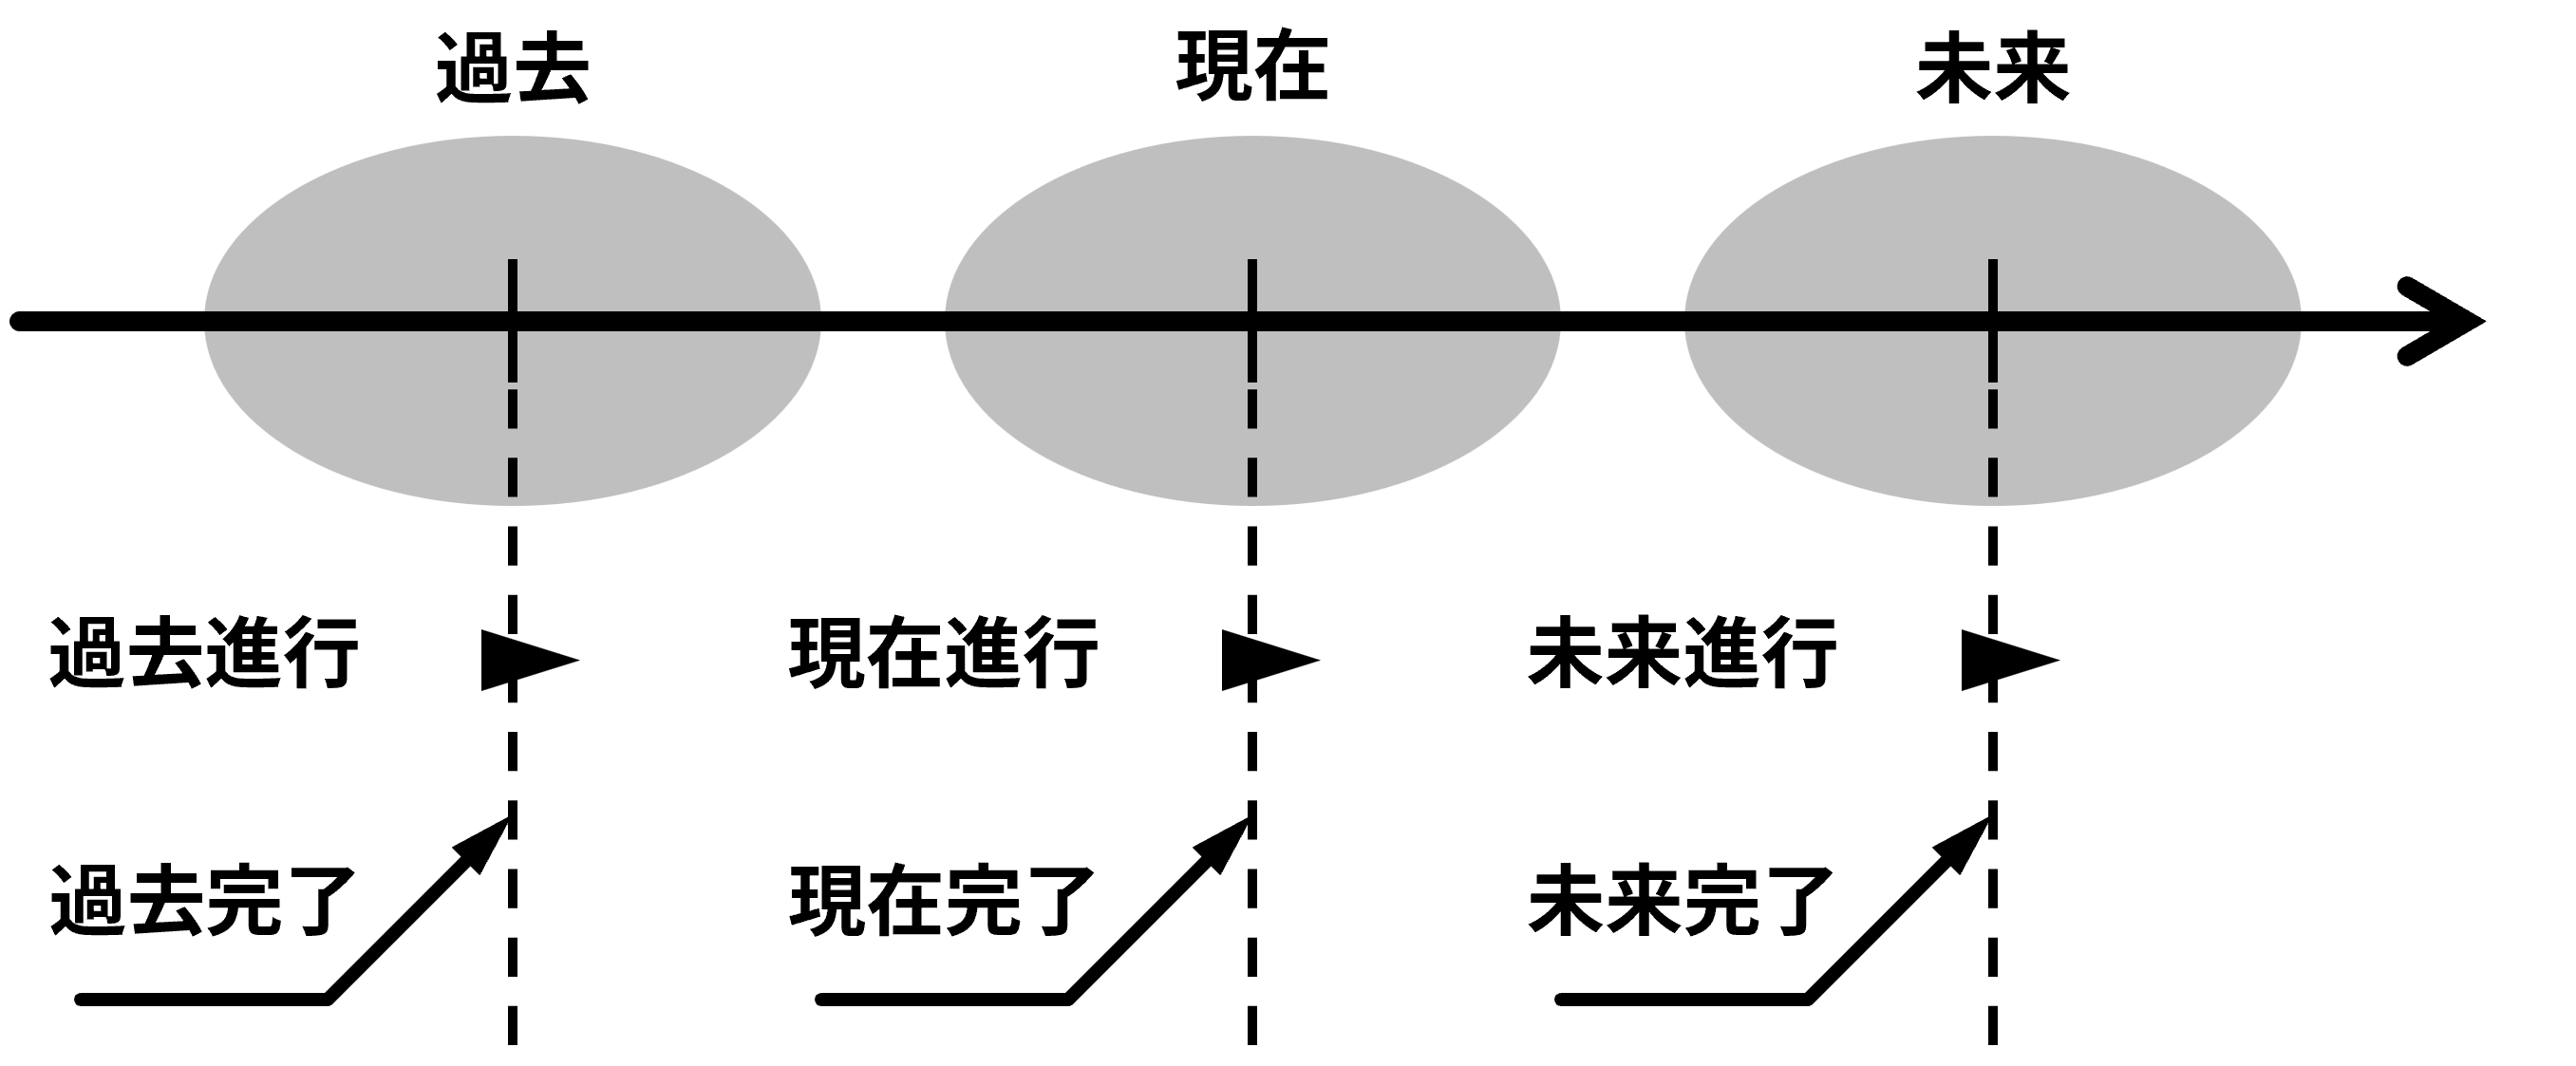
\includegraphics[width=100mm]{fig01.png}
\end{figure}

\subsubsection{現在・過去・未来}

単純な現在は、ざっくりと現在の時点付近のことを述べるのに使う。また、習慣などの反復的な行いや、普遍的な事実について述べるときにも使う。

単純な過去と未来についても、ざっくりとある過去の時点やある未来の時点付近のことを述べるのに使う。

\subsubsection{進行}

進行形は、ある時点で何かの動作や状態が継続しているときに使う。
現在進行形は自明に現在時点についての話だと自明にわかるが、過去進行形と未来進行形はどの時点で進行中なのかを特定させる必要がある。
たとえば、以下の例文を考える。

\begin{align}
  &I ~ am ~ playing ~ the ~ piano \text{.}\\
  &I ~ was ~ playing ~ the ~ piano ~ when ~ my ~ father ~ came ~ home \text{.}\\
  &I ~ will ~ be ~ playing ~ the ~ piano ~ when ~ my ~ father ~ comes ~ home ~ tomorrow \text{.}
\end{align}

どちらも「私はピアノを弾いている最中」であるという文章であるが、一つ目は現在進行形である一方で、二つ目は過去進行形、三つ目は未来進行形である。
後ろの二つでは「どのときに」ピアノを弾いている最中だったのかを示す必要があるため、「父が帰ってきたとき」「明日父が帰ってくるとき」というように過去や未来のどの時点かを特定する文言が入っている。
他にも「昨日の何時」などのように時間を指定する文言が入ることがある。
一方で、単に「昨日」や「先週」というような時間的に幅のある文言が入ることはない。
ちなみに、三つ目のwhen節について、「〇〇するとき」という副詞節のwhen節の中では、たとえ未来のことであっても未来形を使うことができない。
よって、単に現在形での表現になっている。

\subsubsection{完了}

完了には、完了結果・経験・継続の三つの使われ方がある。
どれにも共通していることとしては、「ある時点から見たときの、過去からある時点までの時間の流れ」に着目している点である。
また進行形と同様に、現在完了は現在までについての話だと自明にわかるが、過去完了や未来完了はどの時点までの話なのかを特定させる必要がある。

\paragraph{完了結果}\quad\\

完了結果は、「ある時点でVし終えた」という意味である。

\begin{align}
  &I ~ have ~ finished ~ my ~ homework \text{.}\\
  &I ~ had  ~ finished ~ my ~ homework ~ by ~ dinner ~ yesterday \text{.}\\
  &I ~ will ~ have ~ finished ~ my ~ homework ~ by ~ dinner ~ tomorrow \text{.}
\end{align}

一つ目の文章なら「現時点で」、二つ目と三つ目の文章なら「昨日(明日)の夕食までに」宿題を終わらせているという文章になる。
特に、「ちょうどVした」という意味の$just$、「既にVした」という意味の$already$、「まだVしていない」という意味の$not \sim yet$などと共に使われることが多い。



\subsection{各時制の表し方}

それでは、動詞の活用をおさえたうえで、時制について学ぶ。
時制とは、その文章がどの時点での動作・状態を表すのかというものであり、動詞を活用させたり助動詞を挿入することでそれを表す。

\subsubsection{現在・過去・未来}

\begin{itemize}
  \item 過去\\
  動詞を過去形(Vp)にする。\\
  助動詞がある場合は助動詞を過去形にして動詞を原形に戻す。
  \item 現在\\
  動詞を現在形にする。\\
  助動詞がある場合は助動詞を現在形にして動詞を原形に戻す。\\
  三単現の場合は動詞を三単現の形に活用する。\\
  助動詞がある場合は助動詞を三単現の形に活用して動詞を原形に戻す。\\
  (ただし、三単現の活用がある助動詞は$do \rightarrow does$のみなので、ほとんど考える必要はない)
  \item 未来\\
  助動詞willを挿入する。
\end{itemize}

\subsubsection{進行・完了}

\begin{itemize}
  \item 進行\\
  まず動詞を現在分詞(Ving)に変化させる。\\
  ただ、そうなると活用によって動詞が形容詞となるので、文から動詞がなくなる。\\
  そこで、現在分詞の直前に動詞としてbe動詞を挿入する。\\
  \begin{equation}
    V \rightarrow be + Ving
  \end{equation}
  \item 完了\\
  まず動詞を過去分詞(Vpp)に変化させる。\\
  ただ、そうなると活用によって動詞が形容詞となるので、文から動詞がなくなる。\\
  そこで、現在分詞の直前に動詞としてhaveを挿入する。\\
  \begin{equation}
    V \rightarrow have + Vpp
  \end{equation}
  \item 完了進行\\
  完了と進行の合わせ技をする。\\
  進行形への変化をしてから完了形への変化をすることで完了進行形となる。\\
  \begin{align}
    \begin{aligned}
      V & \rightarrow be + Ving\\
        & \rightarrow have + been + Ving
    \end{aligned}
  \end{align}
\end{itemize}

\subsubsection{複合時制}

現在・過去・未来の3種類と、単純(進行でも完了でもない普通の時制)・進行・完了・完了進行の4種類で、$3 \times 4 = 12$種類の時制が存在する。
それぞれの変形がどのようになるかを以下の表でまとめる。

\begin{table}[h]
  \centering
  \begin{tabular}{clll}
    \hline
     & \multicolumn{1}{c}{過去} & \multicolumn{1}{c}{現在} & \multicolumn{1}{c}{未来}\\
    \hline \hline
    単純 & Vp & V & will V\\
    進行 & be(was/were) Ving & be(is/am/are) Ving & will be Ving\\
    完了 & had Vpp & have Vpp & will have Vpp\\
    完了進行 & had been Ving & have been Ving & will have been Ving\\
    \hline
  \end{tabular}
\end{table}

\subsubsection{文法上の注意点}

ここまで読んで教えてもらった知識と違うと感じる人もいるだろう。
学校教育でもインターネット上の情報でも、はたまた歴史ある辞書でも、完了形のhaveは助動詞として紹介されているからだ。
その代わりに、過去分詞になった動詞を準動詞と呼び動詞として働くものとしている。
これは、意味上の動詞を動詞として扱いたいという考えのもと作られたメソッドである。
当たり前だが、完了形だろうが進行形だろうが意味上の動詞はVのまま変化しない。
だから、過去分詞になったとしてもVppを動詞ライクなものとして扱いたいのだ。
しかし、ここでは分詞になったらもはや動詞ではなくなるという考えのほうを重視し、形式上の動詞としてhaveを置くことにした。
もちろん、この考えにもデメリットがある(後述の疑問形の作り方の部分に影響する)ので、どちらの発想も頭に入れておくに越したことはない。
ややこしい話なので、一旦は「とりあえず完了のhaveは動詞として考えるけど、助動詞的な役割をすることもあるんだな」と思っておいてもらえるとありがたい。




\newpage

\section*{Appendix}

\begin{table}[h]
  \centering
  \begin{tabular}{lll}
    \hline
    \multicolumn{1}{c}{日本語} & \multicolumn{1}{c}{英語(略称)} & \multicolumn{1}{c}{英語}\\
    \hline \hline
    \multicolumn{3}{c}{<品詞>}\\
    名詞 & N. & Noun\\
    代名詞 & Pron. & Pronoun\\
    動詞 & V. & Verb\\
    他動詞 & V.T. & Transitive Verb\\
    自動詞 & V.I. & Intransitive Verb\\
    助動詞 & Aux. & Auxiliary Verb\\
    形容詞 & Adj. & Adjective\\
    副詞 & Adv. & Adverb\\
    接続詞 & Conj. & Conjunction\\
    前置詞 & Prep. & Preposition\\
    冠詞 & & Article\\
    定冠詞 & & Difinite Article\\
    不定冠詞 & & Indifinite Article\\
    間投詞 & Interj. & Interjection\\
    \hline
    \multicolumn{3}{c}{<要素>}\\
    主語 & S & Subject\\
    述語 & V & Verb\\
    目的語 & O & Object\\
    間接目的語 & $\text{O}_1$, IO & Indirect Object\\
    直接目的語 & $\text{O}_2$, DO & Direct Object\\
    補語 & C & Complement\\
    修飾語 & M & Modifier\\
    \hline
  \end{tabular}
\end{table}

\end{document}